\documentclass[11pt,wide]{article}

\usepackage[T1]{fontenc}
\usepackage[utf8]{inputenc}
\usepackage{polski}
\usepackage{lmodern}
\usepackage{amsmath,amsthm}
\usepackage{algpseudocode}
\usepackage{pgfplots}
\usepackage{enumerate}
\newtheorem{thr}{Twierdzenie}
\newtheorem{lem}[thr]{Lemat}
\newtheorem*{dfn}{Definicja}

\title{Analiza numeryczna(M) - Pracownia 1 - Zadanie 18\\
Metody znajdowania pierwiastków funkcji}
\date{Październik 23, 2016}
\author{Wojciech Balik}


\begin{document}

\maketitle                
\thispagestyle{empty}     
\tableofcontents          
\section{Wstęp} 
\subsection{Omówienie tematu}
Wyznaczanie pierwiastków funkcji to problem niewątpliwie ważny dla wielu dziedzin nauki.Jest to też problem trudny ze względu na to że w wielu przypadkach nie potrafimy wyznaczyć miejsc zerowych za pomocą symbolicznych wzorów które potem przekształcimy w konkretną liczbę.\newline
Z pomocą przychodzi nam analiza numeryczna, która oferuje nam szeroką gamę metod wyznaczania rozwiązań przybliżonych, których analizą zajmiemy się w tym sprawozdaniu. Zostanie przytoczone kilka metod numerycznych, lecz więcej uwagi zostanie poświęcone metodzie siecznych, a konkretnie pewnemu jej wariantowi, który w celach czysto praktycznych będziemy nazywać \textit{wariantem A metody siecznych}. Jest to nazwa neutralna, pozwalająca na wyrażanie się o tej metodzie w sposób bardziej rzeczowy
\subsection{Definicje oraz zagadnienia}
Formalnie mówimy że:\newline$x$ jest pierwiastkiem funkcji $f \Leftrightarrow f(x) = 0 $
\newline

\noindent Omawiając dane metody będziemy używać określenia rzędu zbieżności.W tym celu należy wprowadzić kilka podstawowych pojęć:\newline
Niech $\{x_{n}\}$ będzie ciągiem zbieżnym do $\alpha$. Mówimy że $\{x_{n}\}$ zbiega liniowo do $\alpha$ gdy istnieje stała $c \in (0,1)$ i liczba naturalna $N$ takie że:
\begin{equation}
|x_{n+1} - \alpha| \le c|x_n - \alpha| \hspace{1cm} (n \ge N)
\end{equation}
Jeśli istnieje ciąg $\{\epsilon_{n}\}$ zbieżny do 0 i stała $N$ takie że:
\begin{equation}
|x_{n+1} - \alpha| \le \epsilon_{n}|x_n - \alpha| \hspace{1cm} (n \ge N)
\end{equation}
To mówimy że ciąg $\{x_n\}$ zbiega nadliniowo do $\alpha$.\newline
By rozróżnić rodzaje zbieżności nadliniowej, mówimy że rząd zbieżności ciągu $\{x_n\}$ wynosi $p$ jeśli dla pewnych stałych $c \ge 0$ oraz $N$: 
\begin{equation}
|x_{n+1} - \alpha| \le c|x_n - \alpha|^p \hspace{1cm} (n \ge N)
\end{equation}
Warto przypomnieć także twierdzenie Taylora, którego znajomość okaże się przydatna:
\begin{thr}
Załóżmy że funkcja $f$ jest ciągła na przedziale $(a,b)$, posiada ciągłe pochodne aż do rzędu $n$ włącznie, oraz punkty $x$ i $x+h$ należą do przedziału $(a,b)$.Wówczas zachodzi wzór:
\begin{equation}
f(x + h) = f(x) + f'(x)h + f''(x)\frac{h^2}{2!} + f'''(x)\frac{h^3}{3!} + ... + f^{(n-1)}(x)\frac{h^{n-1}}{(n-1)!} + O(h^n)
\end{equation}
\end{thr}
\noindent
(\textbf{Uwaga:} $O(h^n)$ jest jedynie pewnym uproszczeniem, które nam w zupełności wystarcza. Szczegóły, wraz z dowodem można znaleźć w \cite[s.162]{banach}.)




\section{Przegląd wybranych metod wyznaczania pierwiastków funkcji}
\subsection{Metoda Bisekcji}
Fundamentem metody bisekcji jest twierdzenie Darboux(znane także jako twierdzenie Bolzano-Cauchy’ego), które brzmi następująco:
\begin{thr}
Niech $f$ będzie funkcją ciągłą na przedziale $[a,b]$. Jeśli $f(a)f(b) < 0$ to istnieje $c \in [a,b]$ : $f(c) = 0$
\end{thr}
Jeśli dana funkcja $f$ spełnia założenia twierdzenia Darboux, dla $a < b$, to metodę bisekcji można opisać następującym pseudokodem:

\begin{algorithmic}
\While {$|a - b| < \epsilon$}
	\State {$c \gets {\frac{a+b}{2}}$}
	\If {$f(c) = 0$}
		\Return {$c$}
	\EndIf
	\If {$f(c)f(a) < 0$}
		\State {$b \gets c$}
	\Else
		\State {$a \gets c$}
	\EndIf
\EndWhile
\end{algorithmic}

Czyli inaczej mówiąc, dzielimy przedział na pół i aktualizujemy odpowiednio końce przedziału.Jest to metoda niezwykle prosta i intuicyjna,.Niestety, kosztem jej prostoty jest dość wolna zbieżność, albowiem metoda jest zbieżna liniowo. Dowód można znaleźć w \cite[s. 68]{kincaidcheney}

\subsection{Metoda Newtona}
Metoda Newtona(znana również jako metoda stycznych), w przeciwieństwie do metody bisekcji jest na ogół zbieżna kwadratowo.Niestety istnieją przypadki w których jest ona zbieżna liniowo albo wcale nie jest zbieżna, ponadto wymaga ona od nas abyśmy potrafili obliczyć pierwszą pochodną danej funkcji, co nie zawsze jest zadaniem trywialnym.Zakładając również że znamy przybliżenie początkowe $x_0$ pierwiastka funkcji $f$, możemy wyliczyć kolejne przybliżenia następującym wzorem:
\begin{equation}
x_{n+1} = x_n - \frac{f(x_n)}{f'(x_n)}
\end{equation}
Wzór ten wynika z twierdzenia taylora.Załóżmy że $\alpha$ jest pierwiastkiem funkcji $f$. Oznaczmy h = $\alpha - x$. Wtedy:
\begin{center}
$0 = f(\alpha) \approx f(x + h') = f(x) + f'(x)h'$
\end{center}
Co daje nam:
\begin{center}
$h' = -\frac{f(x)}{f'(x)}$
\end{center}
Jeśli dobrze dobierzemy przybliżenie początkowe to $h'$ bedzię dobrym przybliżeniem $h$, więc $x + h'$ będzię lepszym przybliżeniem $\alpha$ \newline
Interpretacja graficzna metody Newtona jest następująca: wyznaczamy styczną do funkcji $f$ w punkcie $x_n$, a jako punkt $x_{n+1}$ obieramy punkt w którym styczna ta przecina oś $OX$. \newline



\begin{tikzpicture}
\begin{axis}[
    xlabel = $x$,
    ylabel = {$f(x)$},
    yticklabels={,,},
    xticklabels={,,},
]
\addplot [
    domain=2.5:4.5, 
    samples=100, 
    color=black,
]
{exp(x) - 25};

\addplot [
	domain=2.5:4.5, 
    samples=100, 
    color=black,
]
{0};

\addplot [
	domain=2.5:4.5, 
    samples=100, 
    color=black,
]
{exp(4)*x - 3*exp(4) - 25};
\addplot [only marks, mark = *, samples at={4}, nodes near coords=$x_n$] {0};
\addplot [only marks, mark = *, samples at={3.457}, nodes near coords=$x_{n+1}$] {0};
\end{axis}
\end{tikzpicture}


Jak już zostało wspomniane, metoda Newtona nie zawsze jest zbieżna. Przykładem może być sytuacja gdy dla pewnego $n$ $f'(x_n) = 0$, wtedy wyraz $x_{n+1}$ będzie nieokreślony. Innym problemem jest to, że dla pierwiastków o parzystej krotności, metoda ta jest zbieżna liniowo. O analizie błędu można doczytać w \cite[s.73]{kincaidcheney}

\subsection{Metoda Siecznych}
\subsubsection{Wariant klasyczny}
Z całą pewnością, wadą metody Newtona jest to że wymaga ona od nas abyśmy umieli obliczać pochodną danej funkcji, której pierwiastki chcemy znaleźć.Jednym ze sposobów na uniknięcie tego jest przybliżenie pochodnej funkcji $f$ za pomocą ilorazu różnicowego:
\begin{center}
$f'(x_n) \approx \frac{f(x_n) - f(x_{n-1})}{x_n - x_{n-1}} $
\end{center}
Zakładając że znamy punkty startowe $x_0$ oraz $x_1$, otrzymujemy wzór:
\begin{equation}
x_{n+1} = x_n - \frac{f(x_n)(x_n - x_{n-1})}{f(x_n) - f(x_{n-1))}}
\end{equation}
(\textbf{Uwaga:} nie zakładamy że $x_{n}x_{n+1} < 0$)\newline
Czyli w przeciwieństwie do metody Newtona, nie wyznaczamy stycznej, lecz sieczną przechodzącą przez punkty $(x_n, f(x_n)$ oraz $(x_{n+1}, f(x_{n+1}))$ i przyjmujemy punkt przecięcia tej stycznej z osią odciętych.Punkty $x_n$ oraz $x_{n-1}$ muszą być takie aby $f(x_n) \neq f(x_{n-1})$.

\begin{tikzpicture}
\begin{axis}[
    xlabel = $x$,
    ylabel = {$f(x)$},
    yticklabels={,,},
    xticklabels={,,},
]
\addplot [
    domain=2.5:7.5, 
    samples=100, 
    color=black,
]
{exp(x) - 25};

\addplot [
	domain=2.5:7.5, 
    samples=100, 
    color=black,
]
{0};

\addplot [
	domain=4.5:7.5, 
    samples=100, 
    color=black,
]
{(exp(7) - exp(6)) * x - 6*exp(7) + 7*exp(6) -  25};

\addplot [only marks, mark = *, samples at={6}, nodes near coords=$x_n$] {0};
\addplot [only marks, mark = *, samples at={7}, nodes near coords=$x_{n-1}$] {0};
\addplot [only marks, mark = *, samples at={5.45}, nodes near coords=$x_{n+1}$] {0};

\end{axis}
\end{tikzpicture}
\newline
\noindent
Niestety, zgodnie z intuicją, jeśli zastąpimy pochodną jej przybliżeniem, to rząd zbieżności nie może się zwiększyć.W rzeczywistości jest wręcz przeciwnie:
\begin{thr}
Rząd zbieżności metody siecznych wynosi $\frac{1 + \sqrt{5}}{2} \approx 1.62$(złota proporcja)
\end{thr}
\begin{proof}
Udowodnione w \cite[s.86]{kincaidcheney}
\end{proof}

\subsubsection{Wariant A}
Używając klasycznej metody siecznych może się zdarzyć tak że przybliżenie $x_{n+1}$ które obliczymy, wcale nie znajduje się bliżej od pierwiastka funkcji którego szukamy, lecz dalej.Dzieje się tak wtedy gdy sieczna którą wyznaczymy jest bardzo "płaska", czyli mówiąc bardziej formalnie, współczynnik kierunkowy prostej opisującej tę sieczną jest (co do modułu) bardzo mały.Nie oznacza to jeszcze rozbieżności, ale jest to na pewno zjawiskiem niepożądanym.

\begin{tikzpicture}
\begin{axis}[
    xlabel = $x$,
    ylabel = {$f(x)$},
    yticklabels={,,},
    xticklabels={,,},
]
\addplot [
    domain=-0.7:1.3, 
    samples=100, 
    color=black,
]
{x^3 + x*x^2 - 0.8};

\addplot [
    domain=-0.7:1.3, 
    samples=100, 
    color=black,
]
{0.23*x - 0.758};

\addplot [
    domain=-0.7:1.3, 
    samples=100, 
    color=black,
]
{0};

\addplot [only marks, mark = *, samples at={-0.25}, nodes near coords=$x_{n-1}$] {0};
\addplot [only marks, mark = *, samples at={0.4}, nodes near coords=$x_n$] {0};


\end{axis}
\end{tikzpicture}

Jednym ze sposobów na naprawienie tego jest sprawdzanie czy kolejne przybliżenie wyznaczone metodą siecznych zbliża nas do szukanego pierwiastka, a gdy tak się nie dzieje, stosowanie bardziej bezpiecznej metody.Taka idea stoi za wariantem A metody siecznych.By go opisać w postaci pseudokodu, wprowadźmy następujące oznaczenia:
\begin{itemize}
\item $MS(x,y)$ - pojedynczy krok metody siecznych dla punktów x,y(dla funkcji której pierwiastków szukamy) 
\item $int(x,y)$ - przedział $(x,y)$ dla $x < y$ lub $(y,x)$ w przeciwnym wypadku.
\end{itemize}

Zakładamy ponadto że punkty $x_0$ oraz $x_1$ są tak dobrane że $f(x_0)f(x_1) < 0$. \newline

\begin{algorithmic}
\State {$a \gets x_0$}
\State {$b \gets x_1$}
\State {$c \gets a$}
\While {$|a - b| < \epsilon$ \textbf{and} $|f(a) - f(b) < \delta$}
	\If {$f(a)f(b) < 0$}
		\State{$b' \gets MS(a,b)$}
	\Else
		\If {$MS(a,b) \in int(b,c)$}
			\State{$b' \gets MS(a,b)$}
		\Else
			\State{$b' \gets \frac{b+c}{2}$}
		\EndIf				
	\EndIf
	\State {$a' \gets b$}
	\If {$f(b)f(b') < 0$}
		\State {$c \gets a$}
	\EndIf
	\State {$b \gets b'$}
	\State {$a \gets a'$} 
\EndWhile
\newline
\Return{$b$}
\end{algorithmic}

\noindent
\newline



\section{Testy numeryczne}
\subsection{Informacje}
Przedstawione wcześniej metody zostały zaimplementowane za pomocą języka Julia(0.5).Testy numeryczne zostały przeprowadzone używając arytmetyki zmiennoprzecinkowej w której na mantysę zostało przeznaczone 256 bitów.Uzyskane przybliżenia zostały porównane z tymi które dostarcza wolframalpha.com. \newline Używana jest notacja:
\begin{itemize}
\item \textbf{MB} - metoda bisekcji
\item \textbf{MN} - metoda Newtona
\item \textbf{MS} - metoda siecznych
\item \textbf{MSA} - metoda siecznych wariant A
\end{itemize}
\subsection{Porównanie}
W poniższych tabelach zostaną przedstawione błędy bezwzględne w kolejnych iteracjach.
\subsubsection{Funkcja $f(x) = e^{sin(x)} - 2x^2 + log(x) + 5x$}

\begin{center}
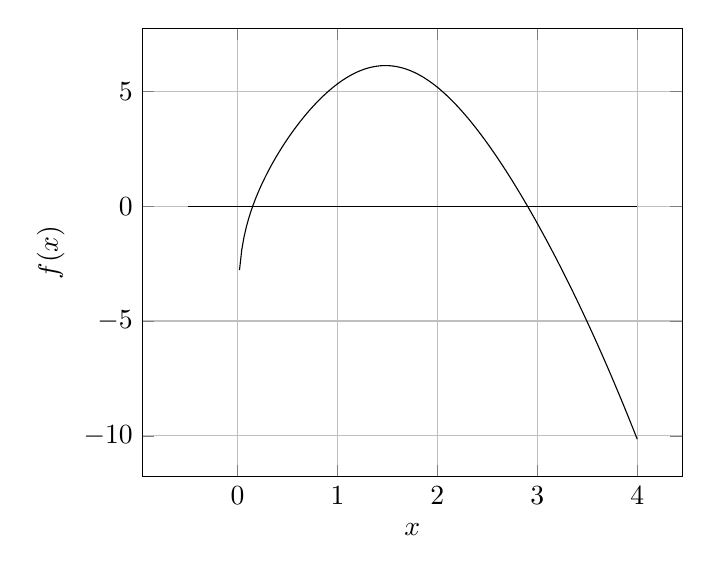
\begin{tikzpicture}
\begin{axis}[
    xlabel = $x$,
    ylabel = {$f(x)$},
    grid = major,
]
\addplot [
    domain=-0.5:4.0, 
    samples=200, 
    color=black,
]
{exp(sin(deg(x))) - 2*(x^2) + ln(x) + 5*x};
\addplot [
    domain=-0.5:4.0, 
    samples=100, 
    color=black,
]
{0};
\end{axis}
\end{tikzpicture}
\end{center}
\noindent
Jako przybliżenia początkowe zostały wybrane $x_0 = 1.7$ dla metody Newtona oraz $x_0 = 1.7 , x_1 = 3.5$ dla metod bisekcji oraz obu wariantów metody siecznych.

\begin{center}
    \begin{tabular}{| c | c | c | c | c |}
    \hline
    Iteracja & MB & MN & MS & MSA \\ \hline \hline
	1 & 4.520e-01 & 2.612e+00 & 3.528e-01 & 3.528e-01 \\ \hline
	2 & 7.300e-02 & 7.331e-01 & 4.340e-02 & 4.340e-02 \\ \hline
	3 & 1.895e-01 & 8.715e-02 & 3.840e-03 & 3.840e-03 \\ \hline
	4 & 5.825e-02 & 1.550e-03 & 3.631e-05 & 3.631e-05 \\ \hline
	5 & 7.372e-03 & 5.162e-07 & 2.995e-08 & 2.995e-08 \\ \hline
	6 & 2.544e-02 & 5.729e-14 & 2.338e-13 & 2.338e-13 \\ \hline
	7 & 9.034e-03 & 7.057e-28 & 1.505e-21 & 1.505e-21 \\ \hline
	8 & 8.311e-04 & 1.071e-55 & 7.567e-35 & 7.567e-35 \\ \hline
	9 & 3.270e-03 & 0.000e+00 & 2.449e-56 & 2.449e-56 \\ \hline
	10 & 1.220e-03 & 3.454e-77 & 3.454e-77 & 3.454e-77 \\ \hline
	11 & 1.943e-04 & 0.000e+00 & 0.000e+00 & 0.000e+00 \\ \hline
	12 & 3.184e-04 & 3.454e-77 & 0.000e+00 & 0.000e+00 \\ \hline
	13 & 6.206e-05 & 0.000e+00 & 0.000e+00 & 0.000e+00 \\ \hline
    \end{tabular}
\end{center}
\noindent
Zgodnie z oczekiwaniami, metoda bisekcji poradziła sobie najgorzej, uzyskując jedynie 5 cyfr dokładnych po trzynastu iteracjach.Oba warianty metody siecznych dały takie same wyniki, co oznacza że nie było potrzeby wykonywania kroku metody bisekcji, stosując wariant A metody siecznych.Inną obserwacją jest to że metoda siecznych jest w stanie konkurować z metodą Newtona dając zadowalające wyniki używając mniej więcej tyle same iteracji, mimo tego że jej rząd zbieżności jest niższy.

\subsubsection{Funkcja: $x - e^{-cos(x)} - \sqrt{log(2 + sin(x))}$}

\begin{center}
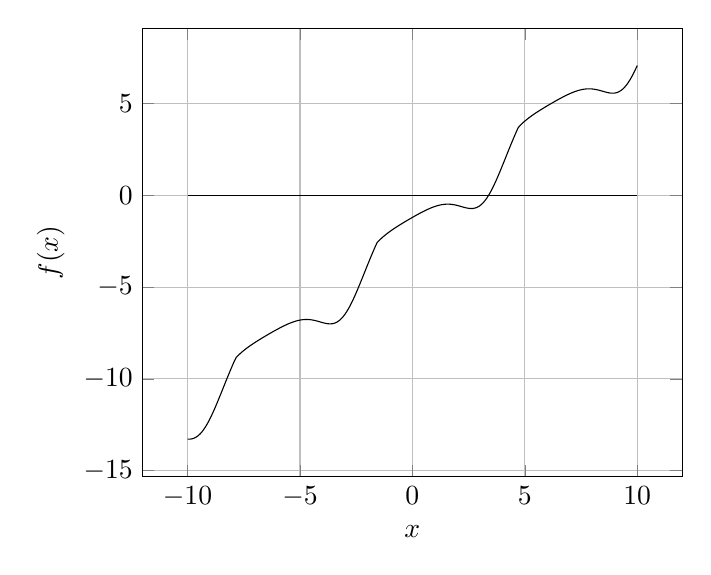
\begin{tikzpicture}
\begin{axis}[
    xlabel = $x$,
    ylabel = {$f(x)$},
    grid=major,
]
\addplot [
    domain=-10:10, 
    samples=250, 
    color=black,
]
{x - exp(-cos(deg(x))) - sqrt(ln(2 + sin(deg(x))))};

\addplot [
    domain=-10:10, 
    samples=100, 
    color=black,
]
{0};
\end{axis}
\end{tikzpicture}
\end{center}
\noindent

Jako przybliżenia początkowe zostały wybrane $x_0 = 2.2$ dla metody Newtona oraz $x_0 = 1 , x_1 = 4$ dla metod bisekcji oraz obu wariantów metody siecznych.

\begin{center}
    \begin{tabular}{| c | c | c | c | c |}
    \hline
    Iteracja & MB & MN & MS & MSA \\ \hline \hline
	1 & 8.879e-01 & 2.936e+00 & 1.569e+00 & 1.569e+00 \\ \hline
	2 & 1.379e-01 & 1.502e+00 & 1.051e+00 & 1.051e+00 \\ \hline
	3 & 2.371e-01 & 3.611e+00 & 3.185e+00 & 2.192e-01 \\ \hline
	4 & 4.960e-02 & 1.729e+00 & 2.522e+00 & 1.964e-01 \\ \hline
	5 & 4.415e-02 & 8.258e+00 & 2.154e+00 & 2.936e-02 \\ \hline
	6 & 2.728e-03 & 4.354e+01 & 1.696e+00 & 3.299e-03 \\ \hline
	7 & 2.071e-02 & 1.578e+01 & 3.815e+00 & 6.691e-05 \\ \hline
	8 & 8.991e-03 & 4.339e+00 & 1.261e+00 & 1.482e-07 \\ \hline
	9 & 3.131e-03 & 5.046e+01 & 7.789e-01 & 6.636e-12 \\ \hline
	10 & 2.015e-04 & 1.553e+01 & 3.547e+00 & 6.582e-19 \\ \hline
	11 & 1.263e-03 & 5.785e+00 & 2.547e+00 & 2.924e-30 \\ \hline
	12 & 5.309e-04 & 3.914e+00 & 2.245e+00 & 1.288e-48 \\ \hline
	13 & 1.647e-04 & 1.824e+00 & 1.755e+00 & 0.000e+00 \\ \hline
    \end{tabular}
\end{center}
\noindent
\noindent
W tym przypadku wyniki nie są takie jakich oczekiwaliśmy.Metoda Newtona oraz metoda siecznych wydają się dawać dość chaotyczne, nie dające żadnego przybliżenia wyniki.W przypadku metody newtona dzieje się to dlatego że punk startowy został wybrany niedaleko pojedynczego miejsca zerowego pochodnej funkcji $f$, przez co wyniki mniej lub więcej oscylują wokół jednego punktu.Metoda siecznych zachowuje się podobnie, ponieważ po pierwszej iteracji, kolejne wyznaczane sieczne bardzo dobrze przybliżają styczną, co prowadzi do podobnego zjawiska jak w metodzie Newtona. Dość dobrze wypada za to wariant A metody siecznych, który dzięki kilku krokom metody bisekcji uzyskał takie punkty $x_n$ oraz $x_{x-1}$ że stosowanie metody siecznych było bezpieczne.\newline
O dziwo, w przypadku metody Newtona oraz metody siecznych, ukazane zjawisko nie prowadzi do rozbieżności.Metoda Newtona zaczęła dawać coraz lepsze przybliżenia od 47 iteracji, a metoda siecznych od iteracji 24, uzyskując dokładność maszynową w iteracjach 53 oraz 36 odpowiednio.

\subsubsection{Funkcja: $\frac{(x-3)(x+1.2)(x-10)(x-3.14) + xlog(x)}{arctg(x) + 2}$}

\begin{center}
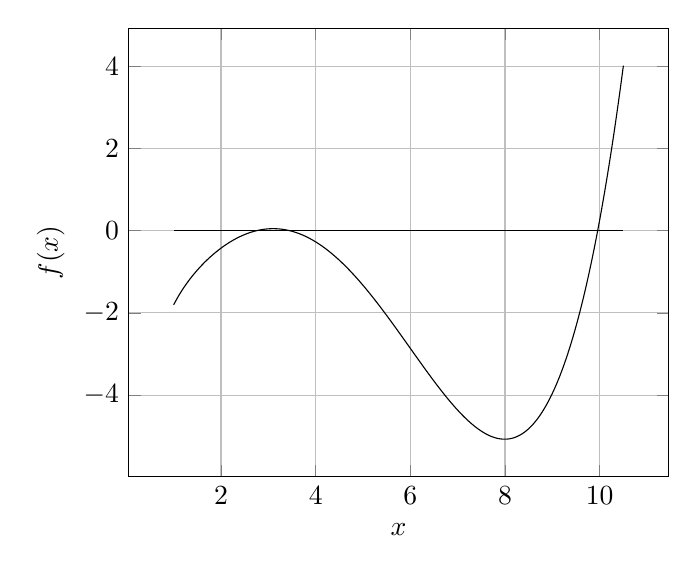
\begin{tikzpicture}
\begin{axis}[
    xlabel = $x$,
    ylabel = {$f(x)$},
    grid=major,
]
\addplot [
    domain=1:10.5, 
    samples=250, 
    color=black,
]
{((x-3)*(x+1.2)*(x-10)*(x-3.14) + x*ln(x))/(atan(x) + 2)};

\addplot [
    domain=1:10.5, 
    samples=100, 
    color=black,
]
{0};
\end{axis}
\end{tikzpicture}
\end{center}
\noindent

Jako przybliżenia początkowe zostały wybrane $x_0 = 3$ dla metody Newtona oraz $x_0 = 3 , x_1 = 4$ dla metod bisekcji oraz obu wariantów metody siecznych.

\begin{center}
    \begin{tabular}{| c | c | c | c | c |}
    \hline
    Iteracja & MB & MN & MS & MSA \\ \hline \hline
	1 & 1.111e-03 & 9.902e-01 & 4.374e-01 & 4.374e-01 \\ \hline
	2 & 2.739e-01 & 7.613e-01 & 2.998e-01 & 2.998e-01 \\ \hline
	3 & 1.364e-01 & 7.048e-01 & 3.074e+00 & 1.246e-01 \\ \hline
	4 & 6.764e-02 & 7.006e-01 & 3.631e-01 & 7.297e-02 \\ \hline
	5 & 3.326e-02 & 7.006e-01 & 4.260e-01 & 1.238e-02 \\ \hline
	6 & 1.608e-02 & 7.006e-01 & 1.646e+00 & 1.510e-03 \\ \hline
	7 & 7.482e-03 & 7.006e-01 & 5.213e-01 & 2.783e-05 \\ \hline
	8 & 3.186e-03 & 7.006e-01 & 5.922e-01 & 6.143e-08 \\ \hline
	9 & 1.037e-03 & 7.006e-01 & 7.453e-01 & 2.504e-12 \\ \hline
	10 & 3.707e-05 & 7.006e-01 & 6.934e-01 & 2.253e-19 \\ \hline
	11 & 5.000e-04 & 7.006e-01 & 7.002e-01 & 8.267e-31 \\ \hline
	12 & 2.315e-04 & 7.006e-01 & 7.006e-01 & 2.729e-49 \\ \hline
	13 & 9.721e-05 & 7.006e-01 & 7.006e-01 & 0.000e+00 \\ \hline
	14 & 3.007e-05 & 7.006e-01 & 7.006e-01 & 3.454e-77 \\ \hline
    \end{tabular}
\end{center}
\noindent
Metoda Newtona oraz metoda siecznych co prawda są zbieżne, ale nie do tego pierwiastka którego sie spodziewaliśmy, co znaczy że należy uważnie dobierać punkty startowe.Waraint A metody siecznych, dzięki użyciu kilku kroków metody bisekcji, znalazł pierwiastek z zadanego zakresu, nie tracąc zbytnio na szybkości zbieżności. Patrząc na wykres funkcji, trzeba zwrócić uwagę że w okolicy punktu $x = 3.4$ funkcja ta przyjmuję wartości dodatnie na dość małym przedziale, co czasami może utrudnić poszukiwanie pierwiastka.

\section{Wnioski}
Zaprezentowany wariant metody siecznych jest bardzo ciekawą alternatywą dla swojego klasycznego odpowiednika, gwarantującą znalezienie pierwiastka na zadanym zakresie, co w teorii skutkuje utratą szybkości zbieżności.W praktyce jednak, zastosowanie jednego bądź jedynie kilku kroków metody bisekcji, często daje nam możliwość wyznaczania kolejnych przybliżeń bardziej efektywnie niż w przypadku gdybyśmy tego nie zrobili.\newline
Minusem wariantu A jest to że nakłada on na nas warunek by funkcja przyjmowała na końcach przedziału różne znaki, czego wariant klasyczny nie wymaga.Może być to problem w przypadku funkcji które przyjmują dany znak na bardzo niewielkim przedziale. Warto także dodać że wariant A wymaga wykonania większej ilości obliczeń(o stałą ilość) od swojego klasycznego odpowiednika.Może to spowolnić czas działania jeśli obliczania wartości funkcji której pierwiastków szukamy jest bardzo kosztowne.
Ogólnie rzecz biorąc, idea stojąca za omawianym wariantem jest bardzo interesująca i z pewnością znalazłaby zastosowanie w bardziej rozbudowanych metodach(np. metoda Brenta) znajdowania pierwiastków równań nieliniowych, w których liczy się odporność na błędy oraz zminimalizowanie potrzeby interwencji użytkownika.


\begin{thebibliography}{10}

\bibitem{kincaidcheney}
  David Kincaid, Ward Cheney,
  przekł. Stefan Paszkowski,
  \emph{Analiza Numeryczna},
  Warszawa, WNT, 2006.
  
\bibitem{banach}
 Stefan Banach,
 \emph{Rachunek różniczkowy i całkowy, Tom I},
 Zakład Narodowy im. Ossolińskich, Lwów, 1929
 

\end{thebibliography}
\end{document}
